Most of the decisions regarding tools were made during implementation.
However the following tool deicisions were made either to aid the design process or were made prior to implementation.
Those made during implementation are outlined in section \ref{sec:impltools}.

\subsection{Trello}
\label{sec:trello}
Trello \citep{trello} is an organisational tool and while it is marketed as a tool to organise anything, it was created initially to organise teams in an office setting with a group of contributors \citep{trellolaunch}.
However it is extremely useful as a project management tool, even for solo projects such as this.

Using Trello, several lists were created to represent different stages of development.
The lists used for the majority of the project were as follows, and an example of these lists in action can be seen in figure \ref{fig:trello}:
\begin{description}
	\item[Backlog] The list of features to be implemented
	\item[Currently Working On] The features currently in development (could be translated to ``current sprint'')
	\item[Stopped: Needs Discussion] The list of features stopped because a design decision needs to be made
	\item[Ready for acceptance] The list of features ready to be shown to and accepted by the stakeholders
\end{description}

\begin{figure}[t]
	\centering
	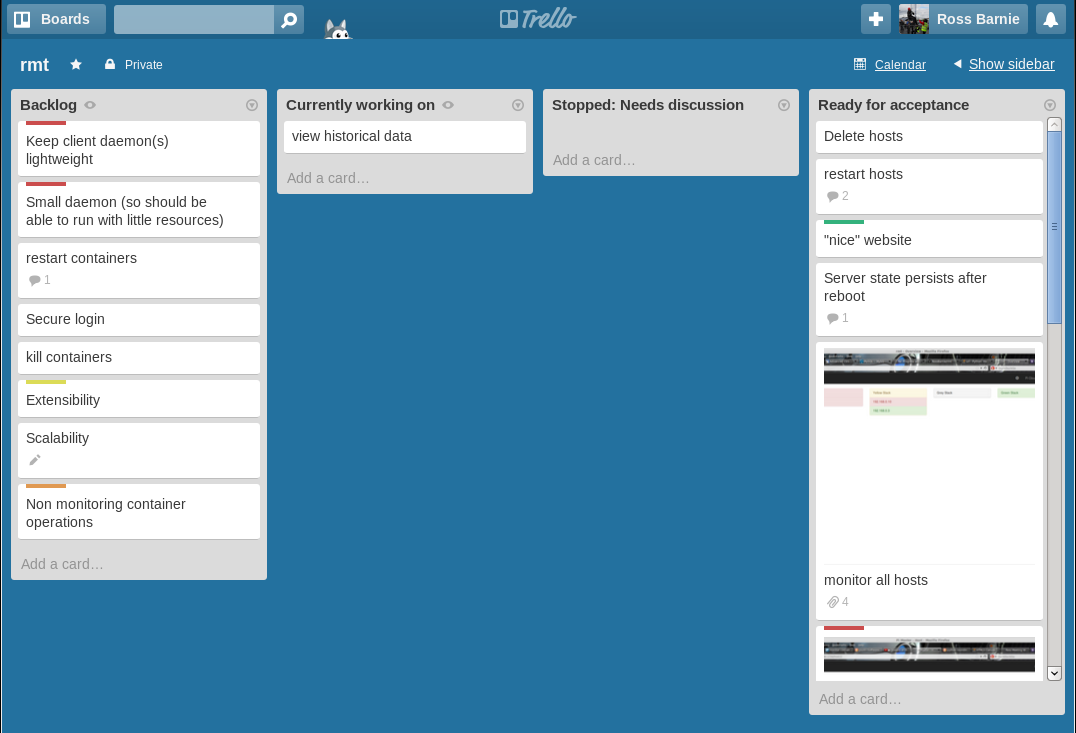
\includegraphics[width=0.8\textwidth]{rmtTrelloCurrent}
	\caption{Example usage of Trello during \emph{rmt} development}
	\label{fig:trello}
\end{figure}

The Trello ``Board'' for the project was also made available to the project supervisor, David White.

As requirements were added, each was given a Trello ``card'' and a priority rating following the MoSCoW priority system, each of which was given a colour, as seen in figure \ref{fig:moscow}.

\begin{figure}[t]
	\centering
	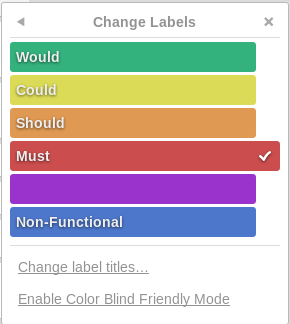
\includegraphics[width=0.3\textwidth]{moscowTrello}
	\caption{MoSCoW priorities as labels in Trello}
	\label{fig:moscow}
\end{figure}

\subsection{git and GitHub}
Version control is a key part of any software development project.
Having previous experience with and an account set up for GitHub \citeyearpar{github}, it was the obvious choice for this project, as well as this document in fact.

The project is currently set to private at \url{http://github.com/RossBarnie/rmt.git} to prevent public interaction however the repository will be made public (ie open-source) once it is no longer required to be developed individually.

\subsection{Python 2.7.6}
Python works very well in a rapid prototyping environment because it allows for applications to be coded quickly and easily, and the language itself is lightweight, catering to that requirement.
Not to mention its excellent documentation and number of different web frameworks available such as Django \citep{django}, webpy \citep{webpy} and web2py \citeyearpar{web2py}, among others.

The legacy version (2.7.6) was chosen over newer versions (latest at time of writing is 3.4.0) because online resources for this version are exhaustive compared to newer versions and because of prior experience with it.

\subsection{Mockingbird}
Mockingbird \citep{mockingbird} is an online diagram creator primarily used to create mock designs of products such as websites or application graphical user interfaces.
In \emph{rmt}, it was used to create a more formal version of designs discussed in meetings.
An example of this can be seen in figure \ref{fig:initialDesign}.

\subsection{JetBrains PyCharm}
PyCharm \citep{pycharm} is a Python Integrated Development Environment (IDE) with many features included to speed up programming in the language, for example:
\begin{itemize}
	\item dark colour scheme
	\item code completion (whereby the editor suggests possible keywords as the user types)
	\item syntax highlighting
	\item line and block commenting
	\item real-time error highlighting
	\item refactoring
	\item remote execution/interpreters
\end{itemize}
This is not an exhaustive list, however these were the features most used in development of \emph{rmt}.
Many of these features can be found in other editors but some, for example GNU Emacs \citeyearpar{emacs}, require setting up of plugins and given that \emph{rmt} would be developed in multiple locations it was very important to be able to easily replicate the development environment with as little configuration as possible.
To that end PyCharm seemed to be the best possible solution since these features were already integrated.

The dark colour scheme is a personal preference however it is much better for developers as they tend to be in front of a computer screen for many hours a day, and a pure white background (such as that found in the Java IDE, Eclipse \citep{eclipse}) can cause eye strain.
Thus it was seen as a priority.

Refactoring in PyCharm is very easy to use and proved useful on a number of occasions in the development of \emph{rmt}.
It allows the developer to change all references to a symbol to something different with minimal input and works on anything from classes to variables.

PyCharm also has remote execution built in.
This allows the developer to use an interpreter on a remote host to run code from the local host, which was used when testing the client application on a Raspberry Pi.
With the Raspbian installation on the Pi used in development having no GUI (which is also true of the hosts in the PiCloud) this was very useful to push code to the Pi without having to commit the code to the repository then pull it on the Pi, speeding up code testing.